\section{Instalasi CodeIgniter3}
\subsection{Kebutuhan Sistem}
Untuk menjalankan CodeIgniter sangat disarankan untuk memakai server dengan PHP tipe 5.4 atau lebih baru. Walaupun keadaan yang sangat memaksa CodeIgniter dapat berjalan pada PHP minimal versi 5.2.4. Menjalankan CodeIgniter pada PHP versi lama sangat tidak dianjurkan, karena dapat memicu gangguan keamanan dan mengurangi fitur yang ada CodeIgniter
\subsection{Langkah-Langkah Instalasi CodeIgniter3}
untuk mengintalasi CodeIgniter, ikuti langkah-langkah berikut ini :
\begin{enumerate}
\item Langkah 1 :
Download CodeIgniter dari https ://codeigniter.com
\item Langkah 2 :
Ekstrak file CodeIgniter-3.1.10.zip ke folder\\
C:
\verb \XAMPP\htdocs \\
\item Langkah 3 :
Rename folder CodeIgniter-3.1.10.zip sesuai dengan yang anda inginkan. untuk contohnya nama dari folder ini akan diubah menjadi folder ci310
\item Langkah 4 :
Didalam folder ci310, terdapat user guide. folder itu berisi tentang dokumentasi atau petunjuk pemakaian CodeIgniter.
\item Langkah 5 :
Jangan lupa kondisi server (XAMPP)  harus aktif , buka halaman http://localhost/ci310/ apabila instalasi codeIgniter berhasil, maka Anda akan mendapatkan tampilan seperti gambar dibawah ini :
\end{enumerate}
\begin{figure}[ht]
\center{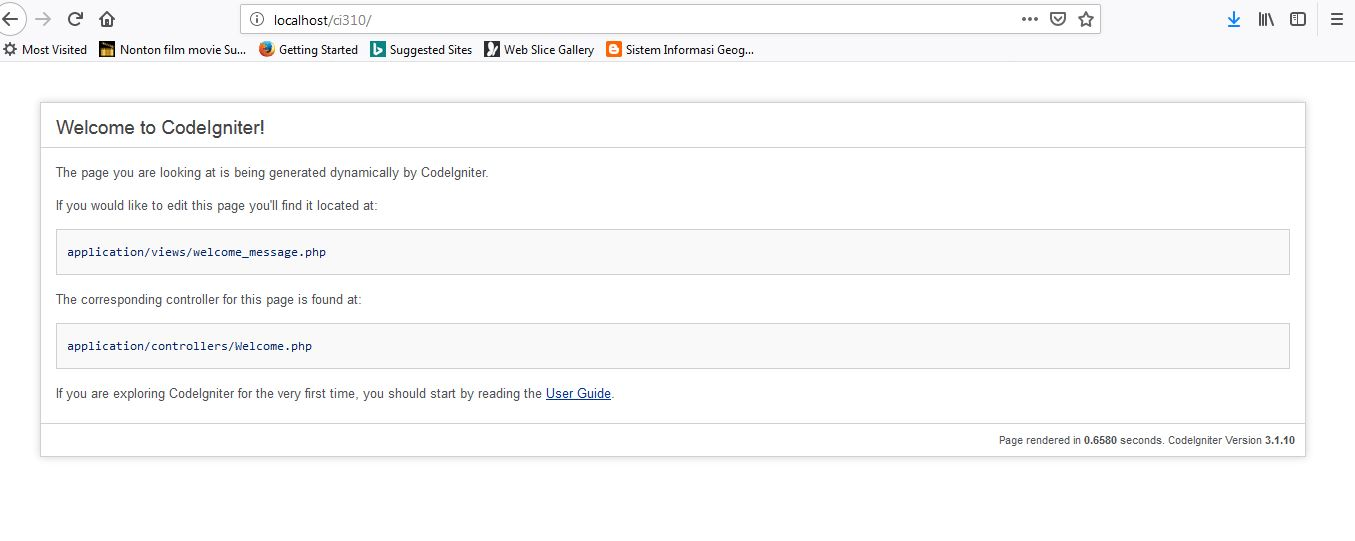
\includegraphics[width=1.0\textwidth]{figures/instalasi.JPG}}
\caption{Halaman Welcome dari CodeIgniter}
\label{Gambar 1}
\end{figure}
